% ============================ Enrico Ribiani 16-03-2021 ====================================================================
% Base per i documenti  
\documentclass[12pt]{article}
% ------------ pacchetti necessari ----------------
\usepackage[a4paper, total={6in, 8in},margin=1in]{geometry} % formattazione decente della pagina
\usepackage{graphicx}                            % need for figure
\usepackage{amsmath}
\usepackage{amsfonts}                            % if you want the fonts
\usepackage{amssymb}                             % if you want extra symbols
 
\usepackage{subfig}
\usepackage{caption}

\renewcommand{\figurename}{Figura}  
\renewcommand{\contentsname}{Indice}                        % need for figures
\usepackage{mathptmx}
%usepackage{float}                               % serve per mettere tabelle e immagini dove si vuole 
\usepackage[utf8]{inputenc}
\usepackage{textcomp}
\usepackage[hang,flushmargin,bottom]{footmisc}   % footnote format
\usepackage{fancyhdr, lastpage}
\usepackage{titlesec}
\usepackage[table,dvipsnames]{xcolor}
%\pagestyle{fancy}
%\renewcommand{\headrulewidth}{0pt}
%\renewcommand*\contentsname{Indice}
\titleformat{\section}{\normalsize\bfseries}{\thesection.}{1em}{}	% required for heading numbering style
\titleformat*{\section}{\Large\bfseries}
\titleformat*{\subsection}{\large\bfseries}
%\usepackage{siunitx}
%\usepackage{tikz}
\usepackage{circuitikz}
%\usepackage[siunitx]{circuitikz}
\usepackage{multirow}
\usepackage{tikz}
\usepackage{amsmath}
\usetikzlibrary{angles,quotes}
\usepackage{placeins}
\usepackage{multirow}
\usepackage{floatrow}
%===================links=================
\usepackage{hyperref}
\hypersetup{
    colorlinks=true,
    linkcolor=Sepia,
    filecolor=Green,      
    urlcolor=Cyan,
    pdftitle={SAMPLE},
    pdfpagemode=FullScreen,
    }
    \usepackage{kvoptions}
    \usepackage{xcolor-material}
    \definecolor{nred}{RGB}{191, 97, 106}
    \definecolor{norange}{RGB}{208, 135, 112}
    \definecolor{nyellow}{RGB}{163, 190, 140}
    \definecolor{ngreen}{RGB}{35, 203, 139}
    \usepackage{colortbl}
    \usepackage{nicematrix}
%===================inizio pagina del titolo=================
\begin{document}
    \begin{titlepage}
    \begin{center}
% ------------------ inizio immagine logo ----------
\begin{figure}
    \centering
    
\includegraphics{~/varie/logo.png}
    \label{fig:logo}
\end{figure}
% ------------------ fine immagine logo ----------
% ------------------ fine immagine logo ----------
-------------------------------------------------------------------------------------\\
\vspace{2\baselineskip}
\large Enrico Ribiani\\
\large 4AUB\\
\vfill

\Huge{\textbf{Esperienza laboratoriale raddrizzatori}}\\
\vfill

\LARGE{esperienza n°5}\\
\vfill
\large{2-12-2021}
\end{center}
%=============== fine pagina titolo ===============
\end{titlepage}
\tableofcontents
\vskip 1cm
\section{Scopo:Verificare il corretto funzionamento di diversi circuiti raddrizzatori.}
    \subsection{Materiale}
    \begin{itemize}
        \item Condensatore $1\mu F$
        \item Condensatore $100 nF$
        \item Resistore da $1k \Omega$
        \item Resistore da $82k \Omega$
        \item Diodo 1N4007
       
        \item cavi per il collegamento
    \end{itemize}
    \subsection{Strumenti}
    \begin{itemize}
        \item Generatore di funzione
        \item Oscilloscopio
        \item Multimetro
    \end{itemize}
    \subsubsection{Schemi}
    \begin{figure}[H]
        \centering
        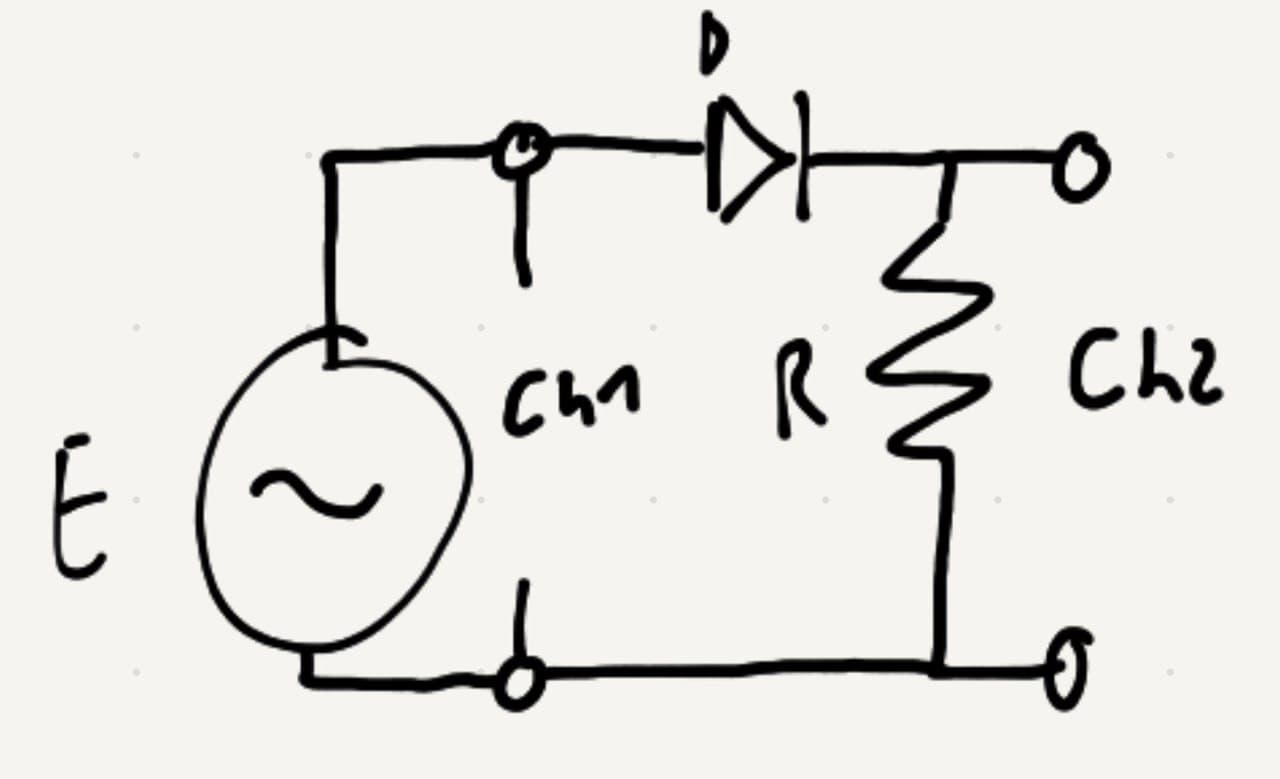
\includegraphics[scale=0.1]{/home/rib/Documenti/latec/Ponte-Graetz/media/r-1s.jpg}          
        \caption{Raddrizzatore}
    \end{figure}
    \begin{figure}[H]
        \centering
        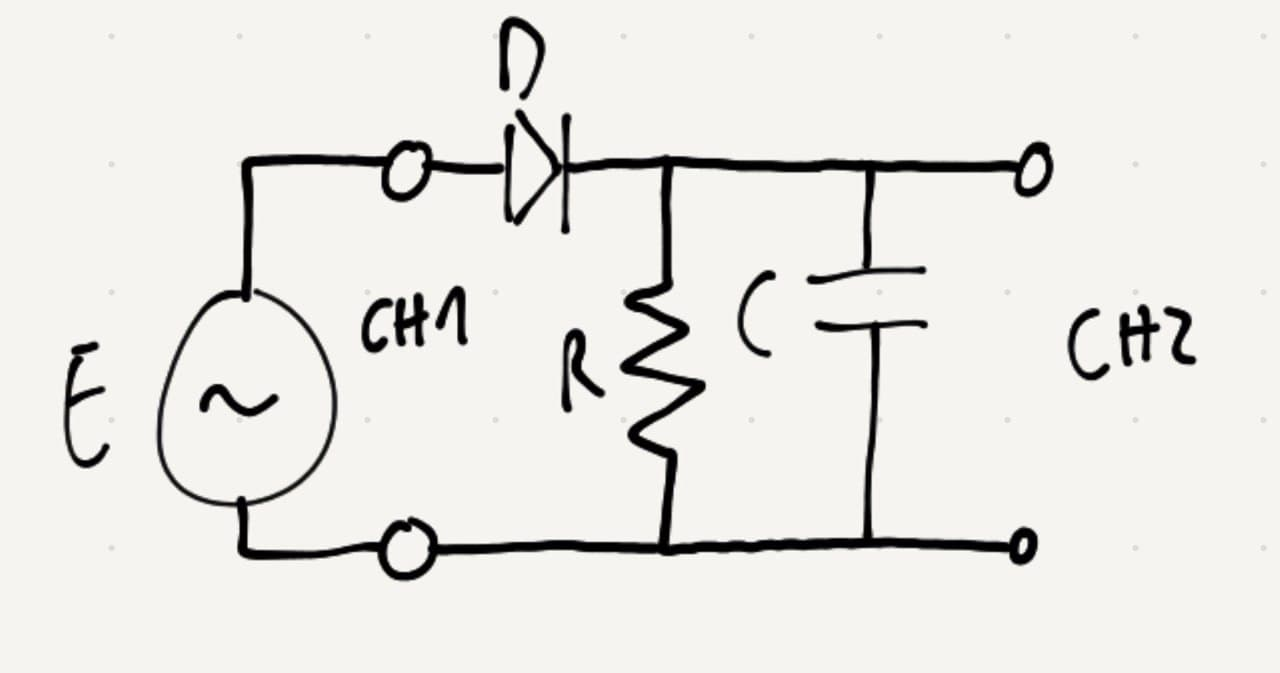
\includegraphics[scale=0.1]{media/rl-1s.jpg}            
        \caption{Raddrizzatore di picco}
    \end{figure}
    \begin{figure}[H]
        \centering
        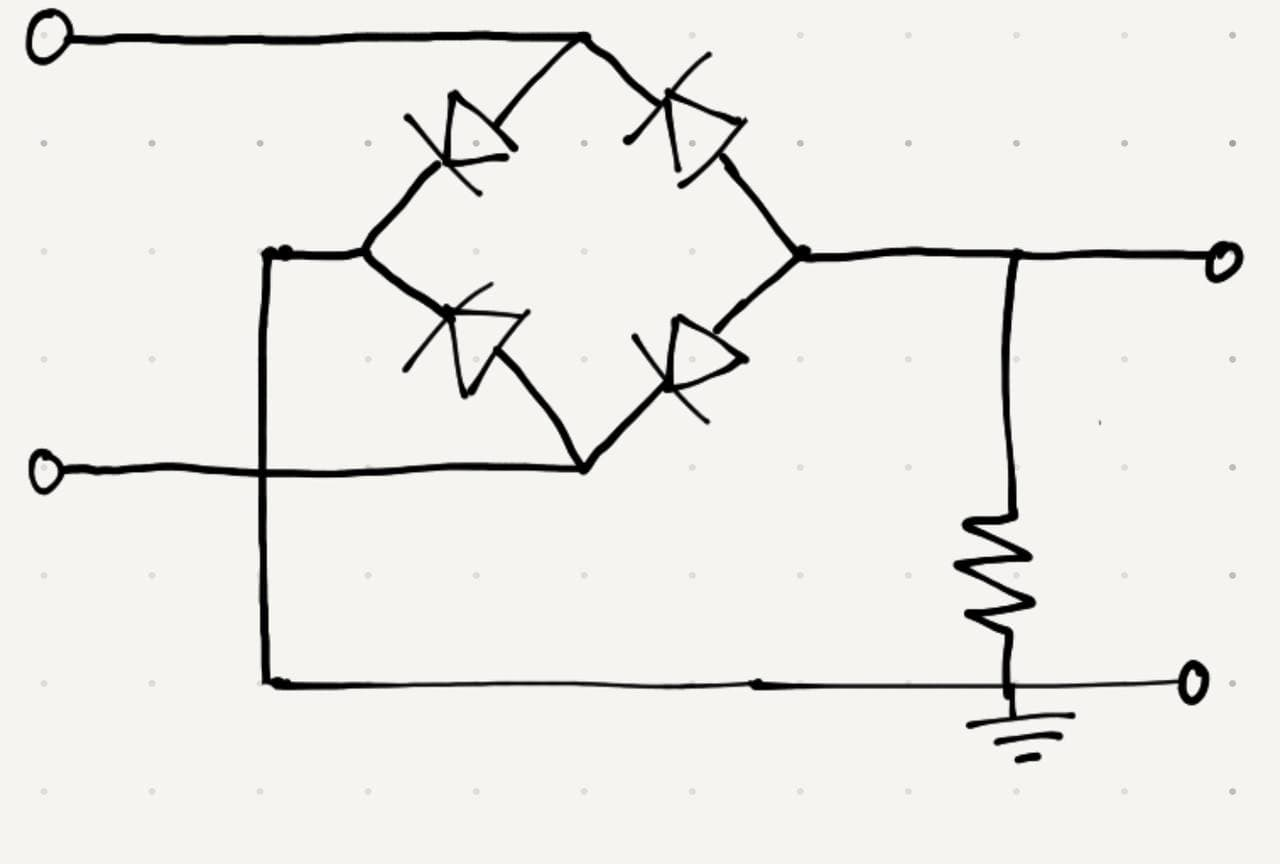
\includegraphics[scale=0.1]{media/pg-schema.jpg}            
        \caption{Ponte di Graetz}
    \end{figure}
    \begin{figure}[H]
        \centering
        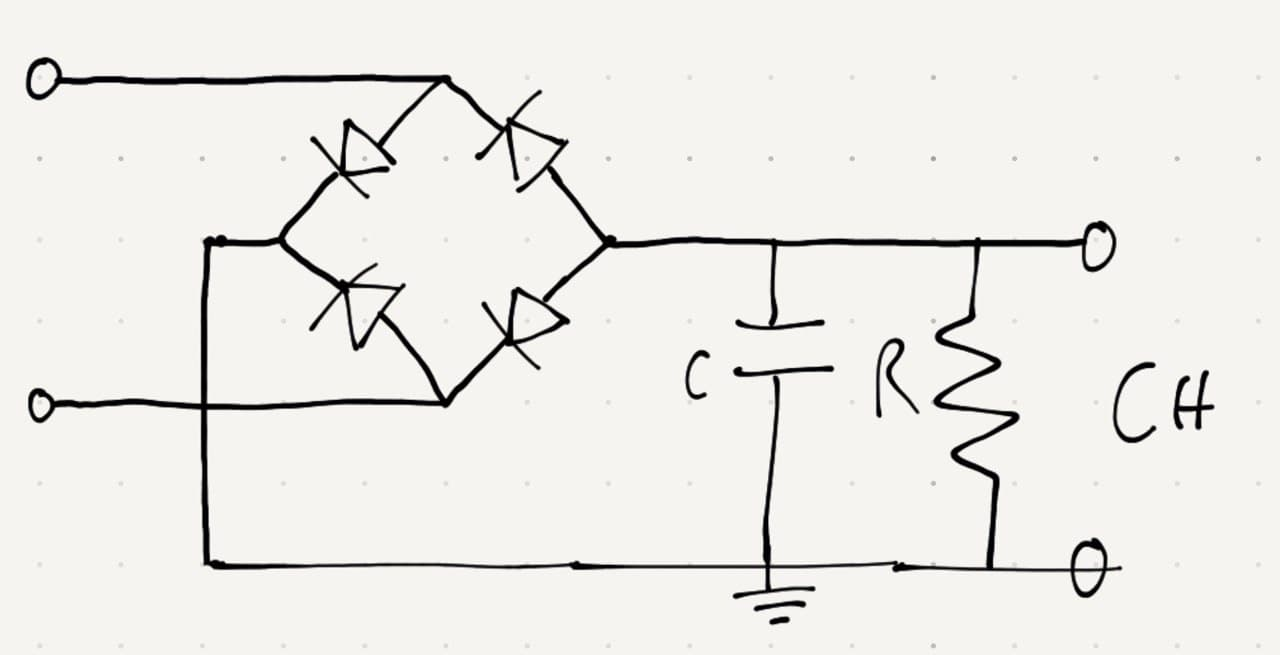
\includegraphics[scale=0.1]{media/pg.jpg}            
        \caption{Ponte di Graetz con condensatore}
    \end{figure} 
     
 
    \section{Cenni teorici}
    \subsection{Raddrizzatore}
    Il circuito raddrizzatore con un diodo andrà a tagliare la parte negativa della sinusoide, se si aggiunge
    un condensatore la parte decrescente della sinusoide positiva andrà a decrescere secondo una retta pendente $\tau$.\\
    Andando ad aumentare R o C la retta sarà meno pendente
    \subsection{Ponte di Graetz}
    Il ponte di graetz serve a convertire la semionda negativa in una positiva diminiuta di due volte $V_s$, aggiungendo un condensatore si
    otterrà lo stesso effetto del raddrizzatore.
    \section{Procedimento}
    Procediamo a montare il circuito, si regola il generatore di fuonzione a 5Vp con 100Hz, dopodichè si va a mettere i puntali dell'oscilloscopio
    seguendo lo schema. Si procede osservando l'effetto del circuito sulla tensione in ingresso.\\
    Per i circuiti limitatori di picco si procede a misurare il ripple.\\
    \section{Conclusioni}
    \begin{figure}[H]
        \centering
        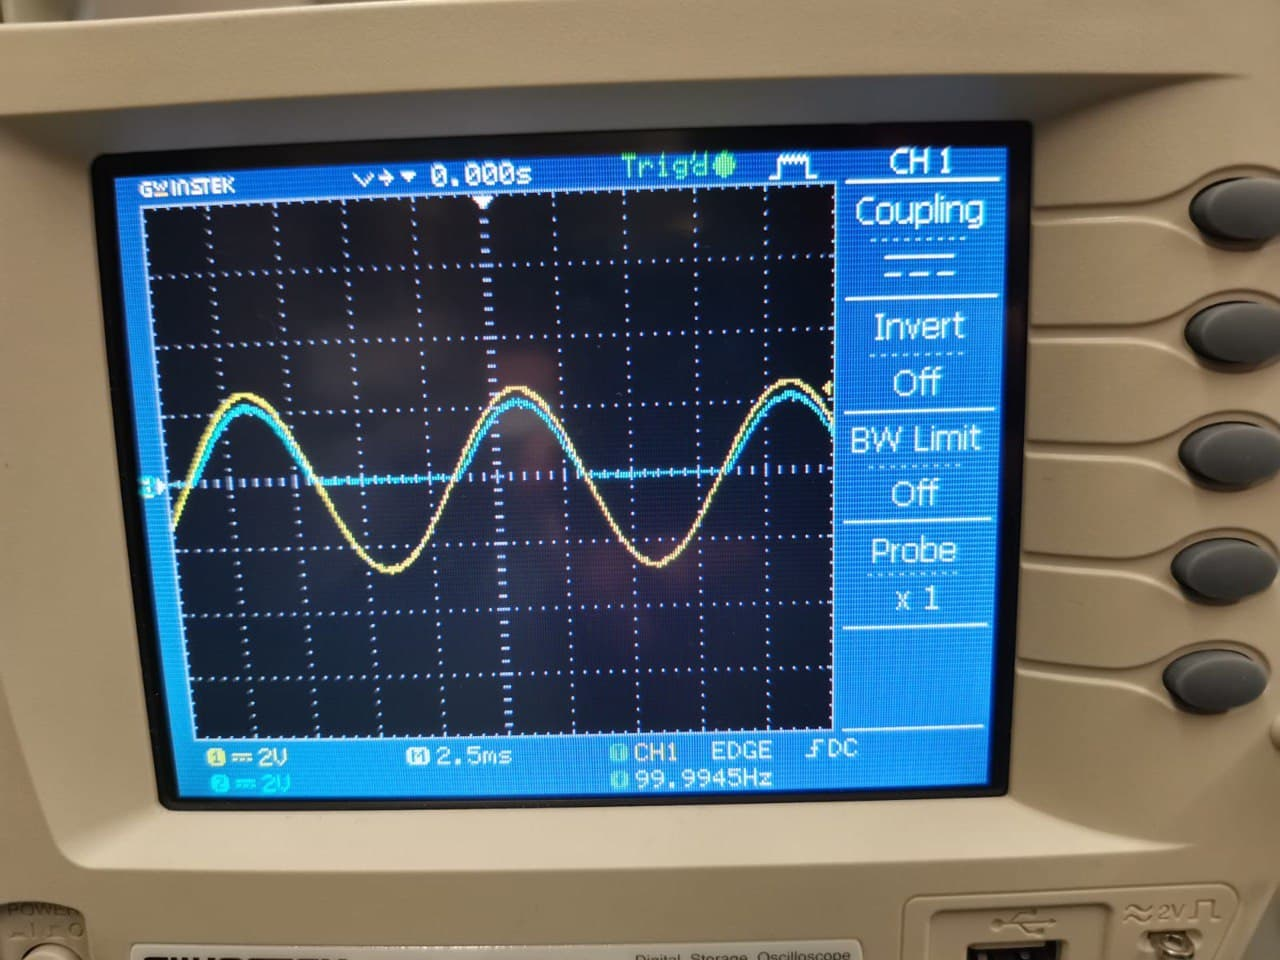
\includegraphics[scale=0.1]{media/r-1s-osc.jpg}       
        \caption{Raddrizzatore}   
    \end{figure}
    I cenni teorici sono stati verificati
    \begin{figure}[H]
        \centering
        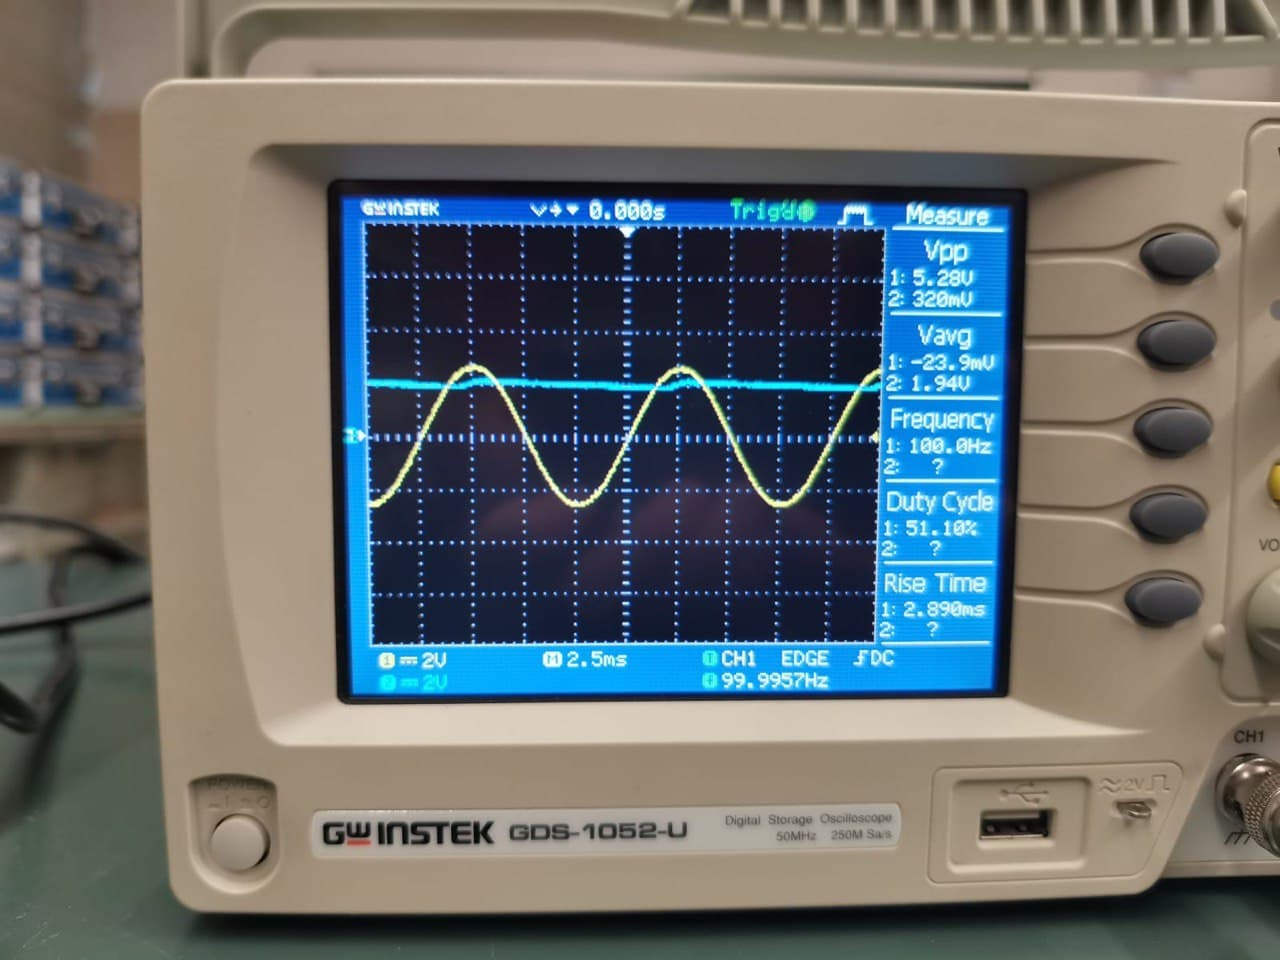
\includegraphics[scale=0.1]{media/rc-1.jpg}
        \caption{Raddrizzatore di picco con 1$\mu$F}          
    \end{figure}
    I cenni teorici sono stati verificati
    \begin{figure}[H]
        \centering
        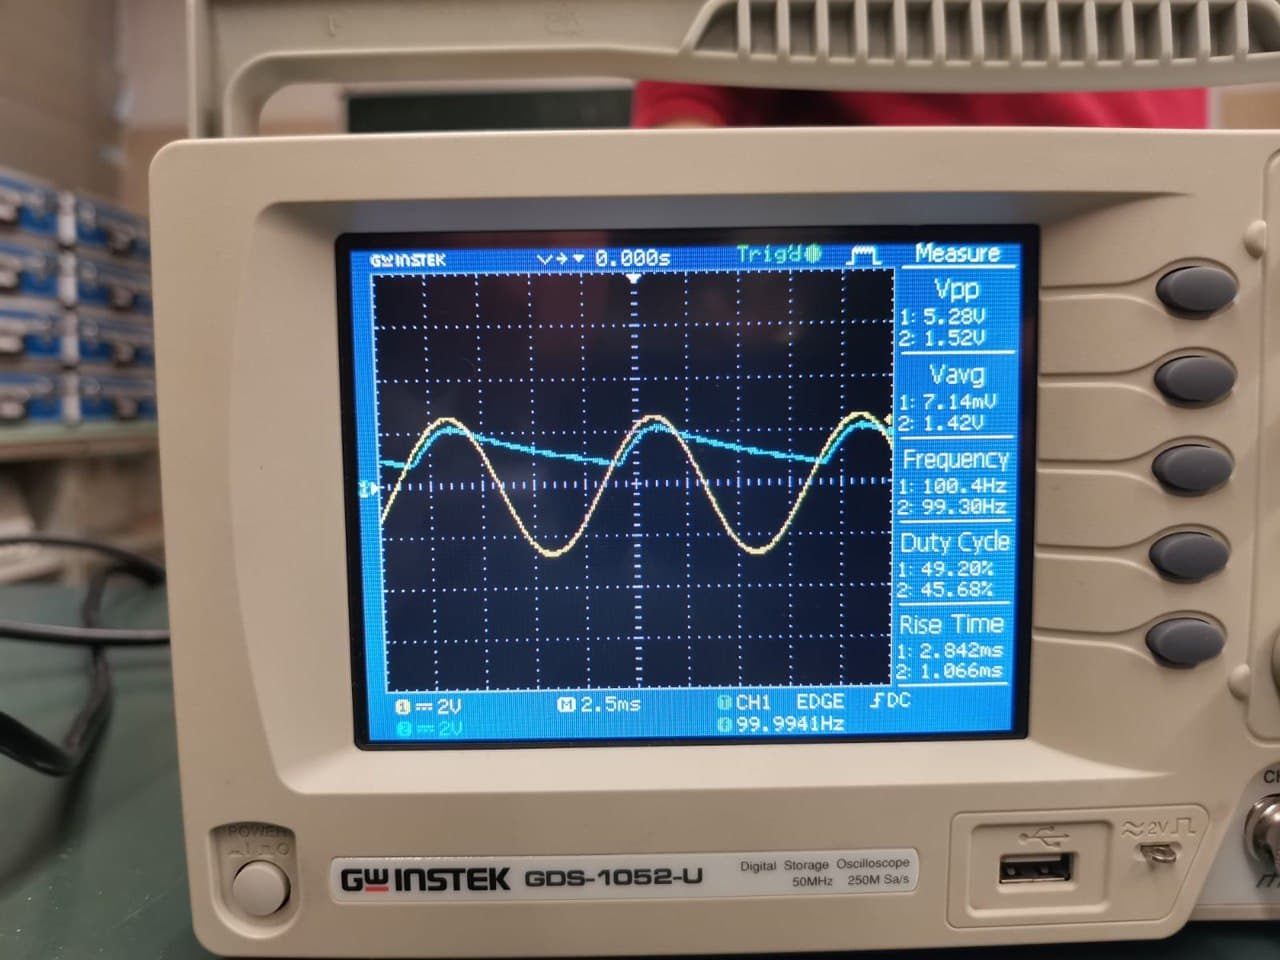
\includegraphics[scale=0.1]{media/rc-100.jpg}   
        \caption{Raddrizzatore di picco con 100nF}          
    \end{figure}
    I cenni teorici sono stati verificati, il ripple è di 2,8V\\
    \begin{figure}[H]
        \centering
        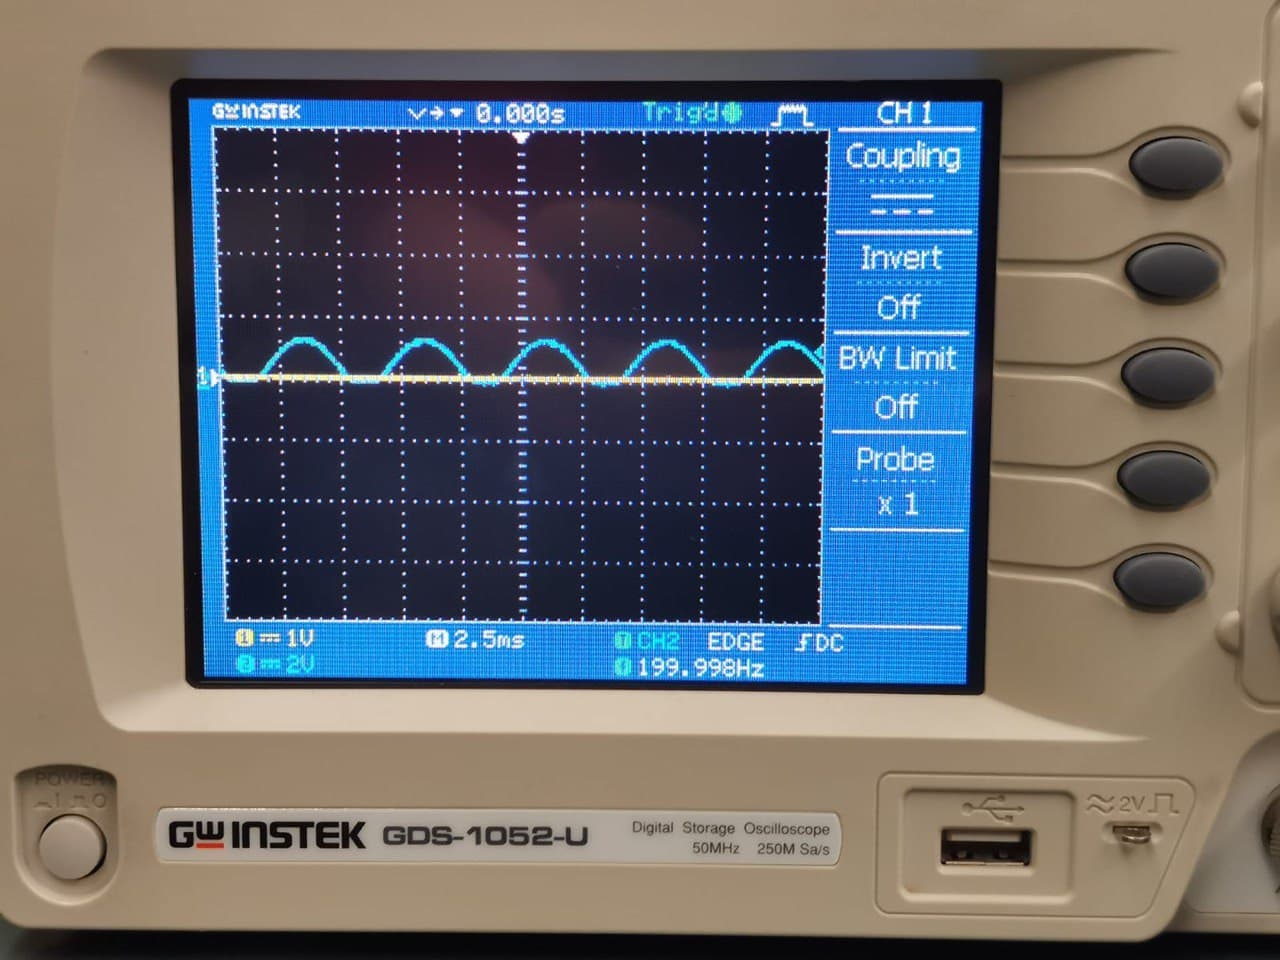
\includegraphics[scale=0.1]{media/pg-osc.jpg}       
        \caption{Ponte di Graetz}   
    \end{figure}
    I cenni teorici sono stati verificati, il ripple è di 480mV\\
    \begin{figure}[H]
        \centering
        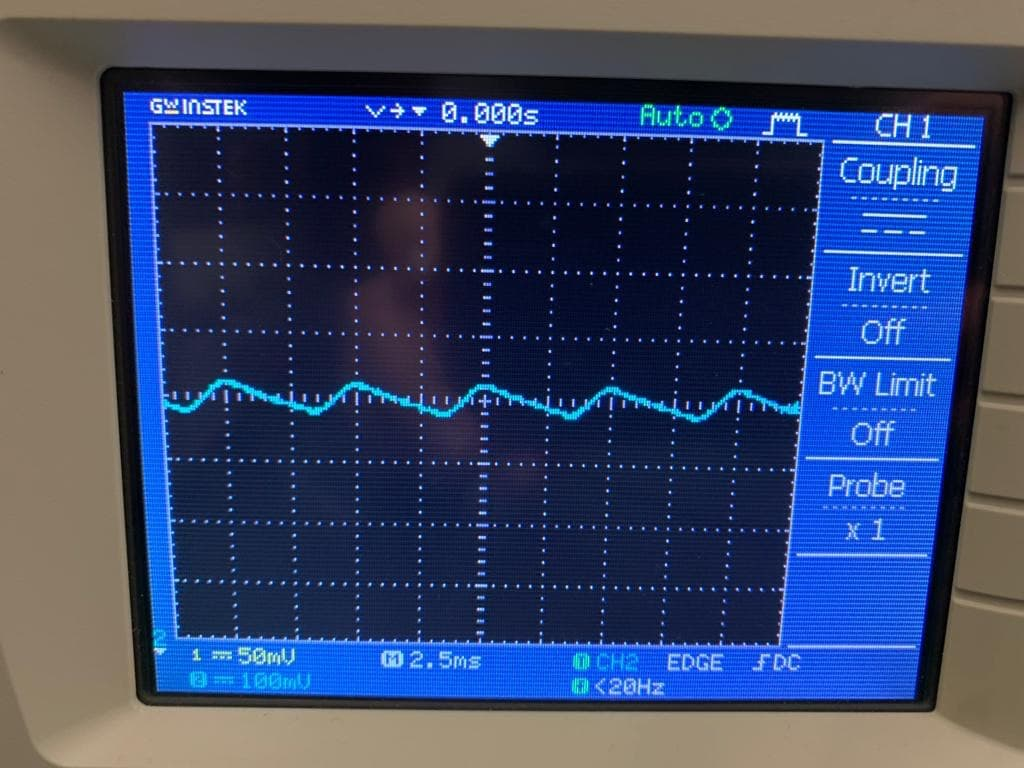
\includegraphics[scale=0.1]{media/pgc-osc.jpg}       
        \caption{Ponte di Graetz con condensatori}   
    \end{figure}
    \noindent I cenni teorici sono stati verificati, l'onda di uscita risulta come una specie di onda a dente di sega\\
\end{document}
